% TU Delft beamer template
% Author: Erwin Walraven (initial version was created by Maarten Abbink)
% Delft Universiy of Technology

\documentclass{beamer}
\usepackage[english]{babel}
\usepackage{calc}
\usepackage[absolute,overlay]{textpos}
\usepackage{graphicx}
\usepackage{subcaption}
\captionsetup[figure]{font=scriptsize,labelfont=scriptsize}
\captionsetup[subfigure]{font=scriptsize,labelfont=scriptsize}
\usepackage{amsmath}
\usepackage{amsfonts}
\usepackage{amsthm}
\usepackage{mathtools}
\usepackage{comment}
\usepackage{MnSymbol,wasysym}

\setbeamertemplate{navigation symbols}{} % remove navigation symbols
\mode<presentation>{\usetheme{tud}}

% BIB SETTINGS
%\usepackage[backend=bibtex,firstinits=true,maxnames=30,maxcitenames=20,url=false,style=authoryear]{biblatex}
%\bibliography{bibfile}
%\setlength\bibitemsep{0.3cm} % space between entries in the reference list
%\renewcommand{\bibfont}{\normalfont\scriptsize}
%\setbeamerfont{footnote}{size=\tiny}
%\renewcommand{\cite}[1]{\footnote<.->[frame]{\fullcite{#1}}}


\title[]{Transiently-powered Battery-free Robot}
\institute[]{Delft University of Technology}
\author{Koen Schaper}
%\date{}

\logo{
\includegraphics[width=3cm]{pics/es_logo_cyan_black_rgb}}

\begin{document}
{
\setbeamertemplate{footline}{\usebeamertemplate*{minimal footline}}
\frame{\titlepage}
}

{\setbeamertemplate{footline}{\usebeamertemplate*{minimal footline}}

}

\begin{frame}{Overview}
		Introduction \\
		\vspace{1em}
		Design and Implementation
		\begin{itemize}
			\item Hardware
			\item Control
			\item Software
		\end{itemize}
		Evaluation \\
		\vspace{1em}
		Conclusion
\end{frame}

\begin{frame}{Small robotic platforms}
	\begin{figure}
		\begin{subfigure}[b]{0.32\textwidth}
			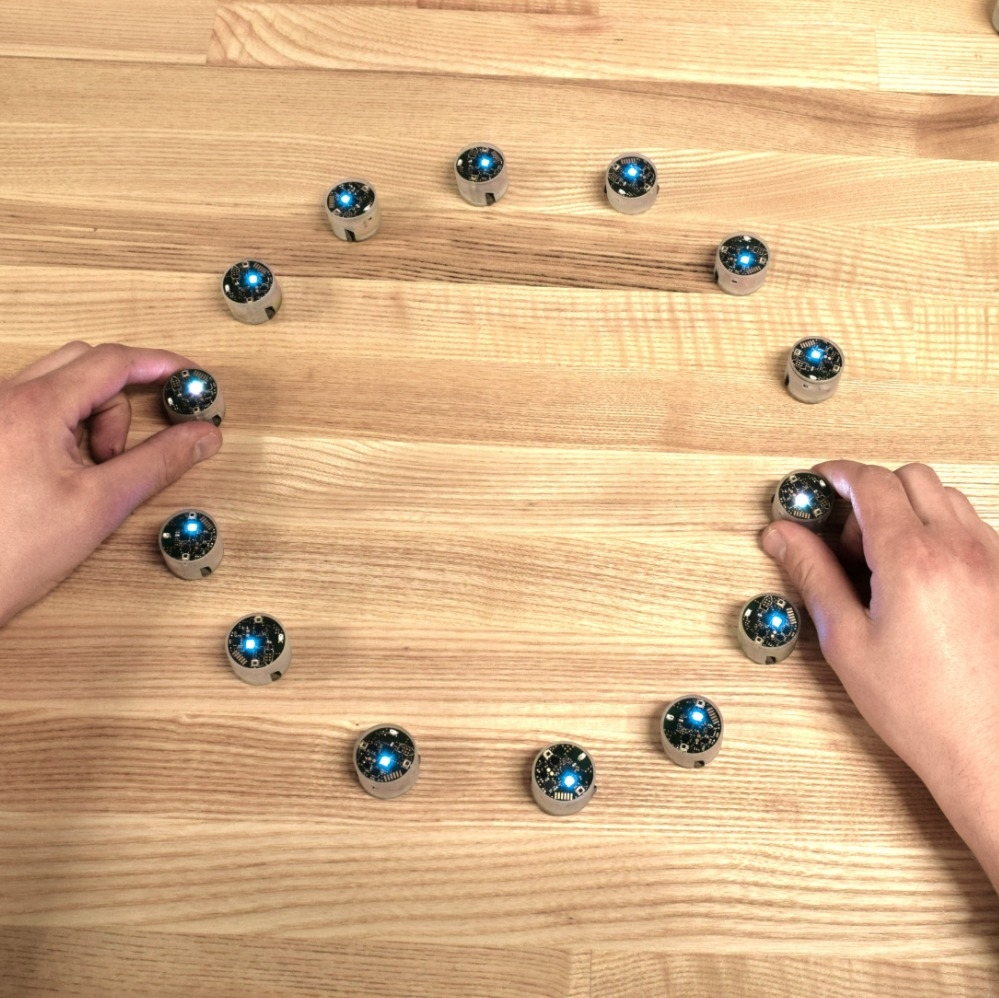
\includegraphics[width=\textwidth]{pics/zooids.jpg}
			\caption*{Zooids}
		\end{subfigure}
		\begin{subfigure}[b]{0.324\textwidth}
			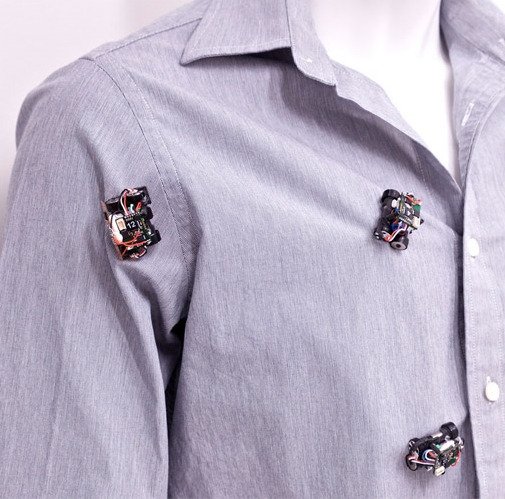
\includegraphics[width=\textwidth]{pics/rovables.jpg}
			\caption*{Rovables}
		\end{subfigure}
		\begin{subfigure}[b]{0.323\textwidth}
			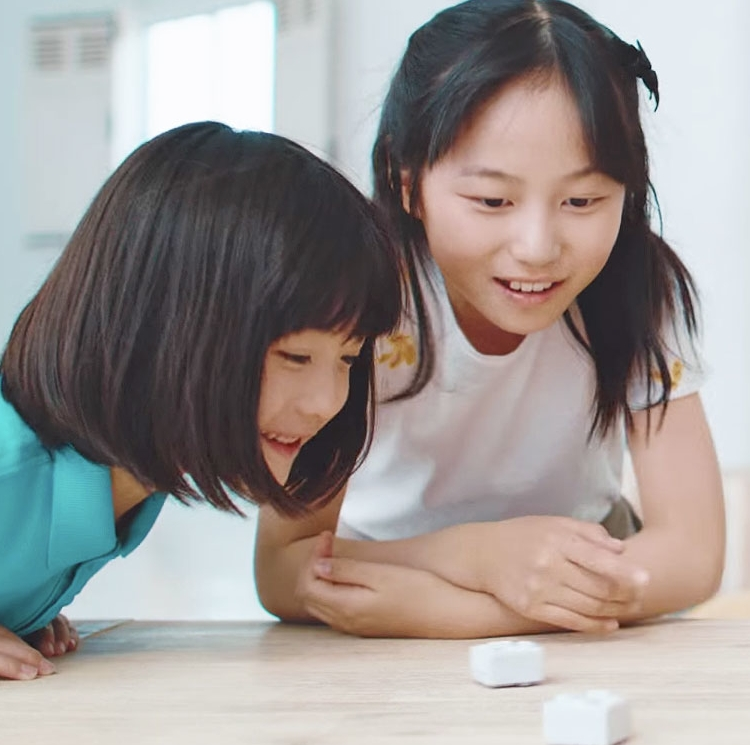
\includegraphics[width=\textwidth]{pics/toio.jpg}
			\caption*{Sony Toio}
		\end{subfigure}
	\end{figure}
	Operation time is limited by Li-ion batteries
\end{frame}

\begin{frame}{Problem of batteries}
	New battery technologies
	\begin{itemize}
		\item Overhyped and slow emerging
	\end{itemize}
	\vspace{0.5em}
	Replenishment methods
	\begin{itemize}
		\item Recharging or battery replacement
	\end{itemize}
	\vspace{2em}
	\pause
	\textbf{Solution:} \\
	Energy from ambient sources stored in capacitors
\end{frame}

\begin{frame}{Energy harvesting}
	%\vspace{1em}
	\begin{figure}
		\centering
		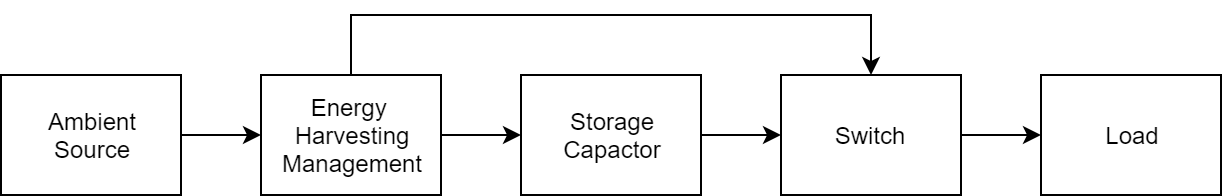
\includegraphics[width=0.8\textwidth]{pics/Harvesting-diagram.png}
	\end{figure}
	%\pause
	\begin{minipage}{0.45\textwidth}
		\textbf{1000x} smaller energy storage \\\\
		\textbf{Challenge}: \\
		Frequent power interrupts
	\end{minipage}
	\begin{minipage}{0.54\textwidth}\raggedleft
		\begin{figure}
			\vspace{2em}
			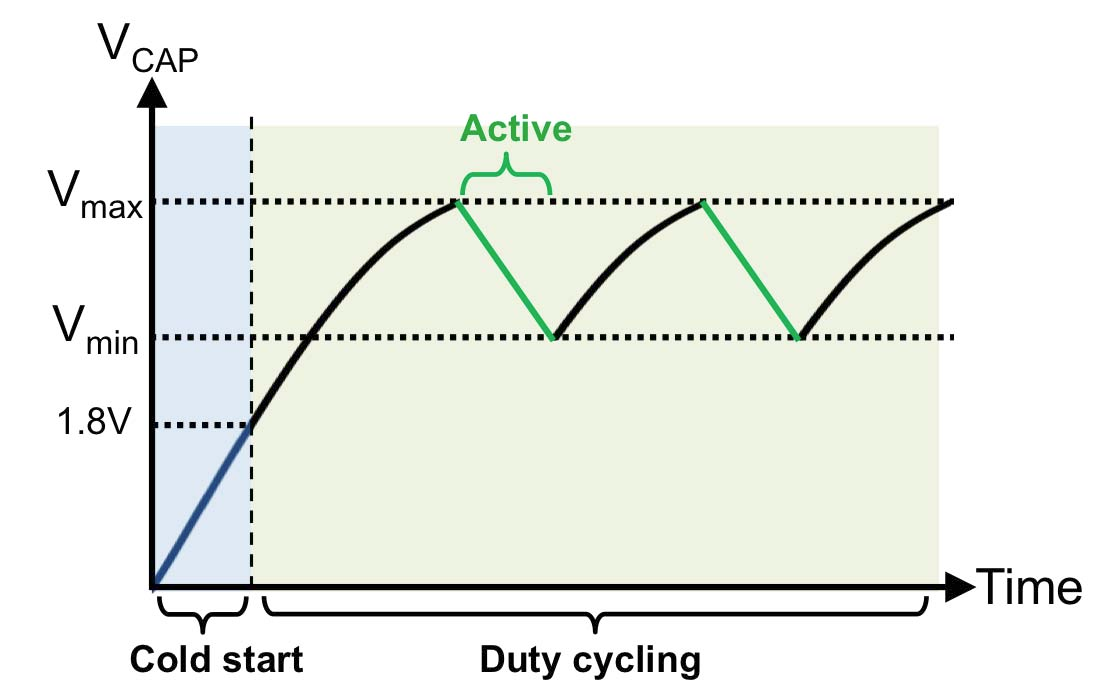
\includegraphics[width=0.9\textwidth]{pics/Voltage_time_harvester.png}
			\caption*{Image: Naderiparizi RFID' 15}
		\end{figure}
	\end{minipage}
\end{frame}

\begin{frame}{Research question}
	\begin{center}
	%\begin{block}{}
		What is the effect of intermittency on the movement accuracy of a transiently-powered robot without external feedback?
	%\end{block}	
	\end{center}
\end{frame}

\begin{frame}{Design requirements}
	Power \\
	\begin{itemize}
		\item Not rely on batteries
	\end{itemize}
	Small form factor \\
	\begin{itemize}
		\item Lower material cost
	\end{itemize}
    Locomotion \\
    \begin{itemize}
    	\item Efficient actuator for movement
    \end{itemize}
    Controlled movements \\
    \begin{itemize}
    	\item Complete movement across power cycles
    \end{itemize}
\end{frame}

\begin{frame}{Power}
	\vspace{1em}
	\begin{minipage}{0.45\textwidth}
		Energy from light \\
		
		Solar panel \\
		
		\textbf{6\,s} Charge time \\
		
		\textbf{1\,s} Operation time \\
		
	\end{minipage}
	\begin{minipage}{0.54\textwidth}\raggedleft
		\begin{figure}
			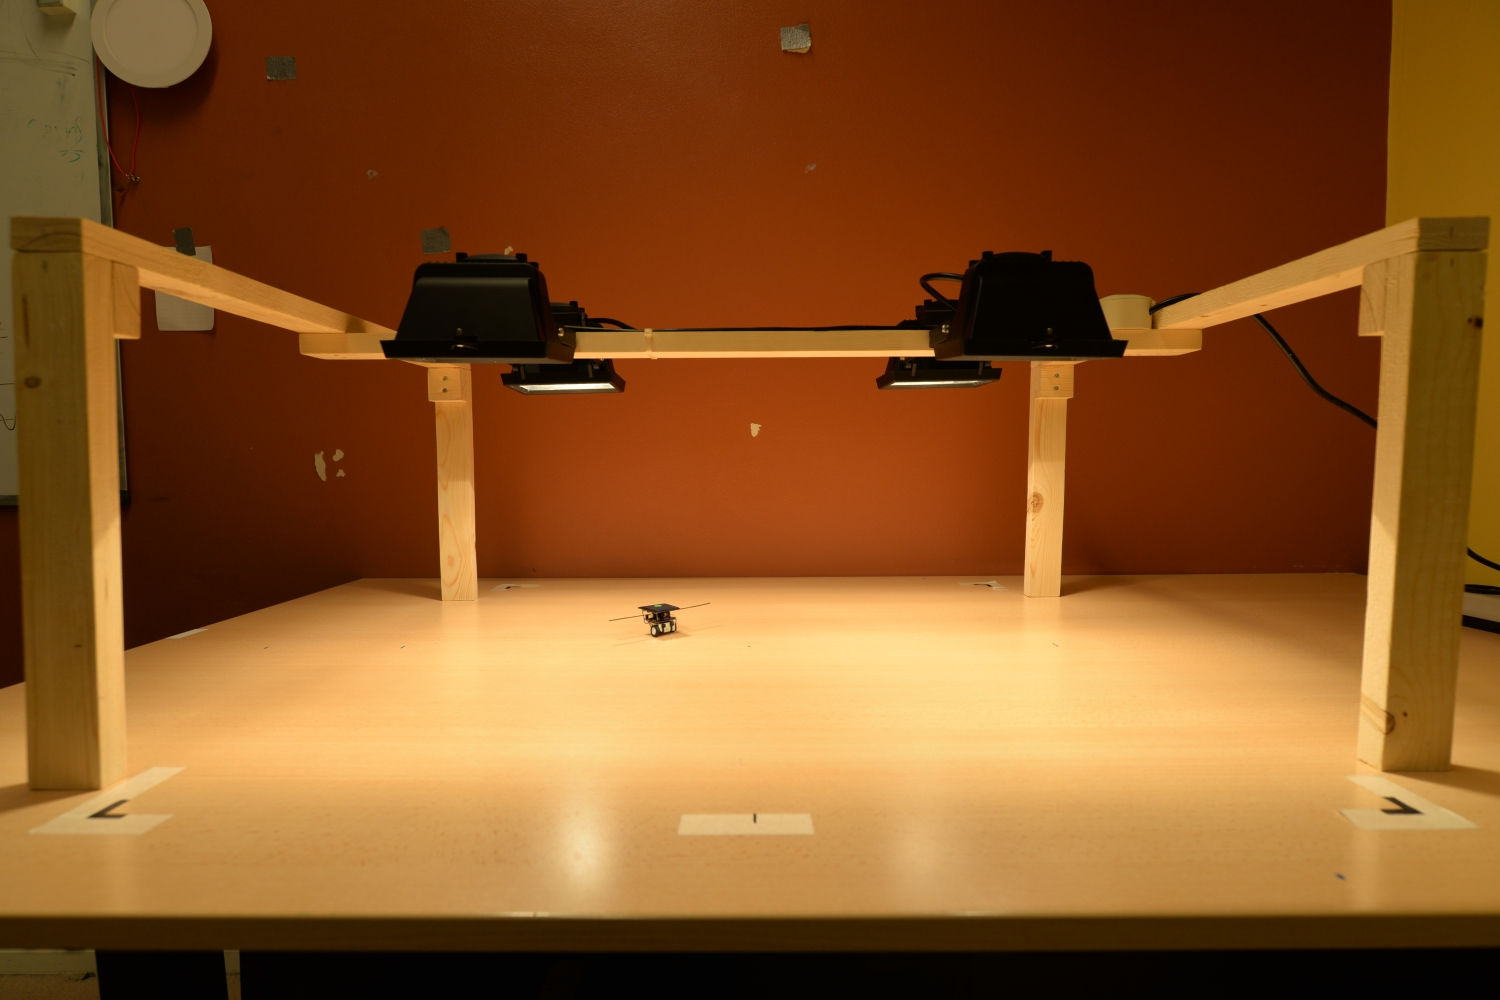
\includegraphics[width=0.9\textwidth]{pics/light_setup.jpg}
			\caption*{Light setup}
		\end{figure}
	\end{minipage}
\end{frame}

\begin{frame}{Locomotion}
	\begin{minipage}{0.45\textwidth}
		Geared DC motors \\
		
		Start current peak \\
		
		Maximum current harvester: \\
		110\,mA
	\end{minipage}
	\begin{minipage}{0.54\textwidth}\raggedleft
		\begin{figure}
			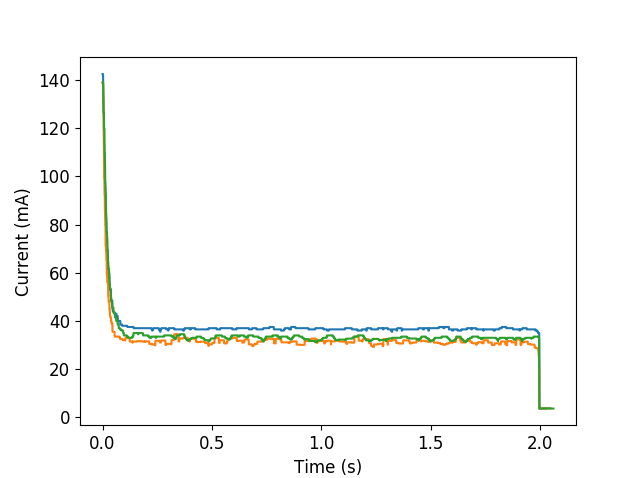
\includegraphics[width=\textwidth]{pics/free_running_current.png}
			\caption*{DC motor current profile}
		\end{figure}
	\end{minipage} \\
	\pause
	\vspace{1em}
	\textbf{Solution:} Pulse Width Modulation + Bulk capacitor
\end{frame}

\begin{frame}{Schematic overview}
	\begin{figure}
		\centering
		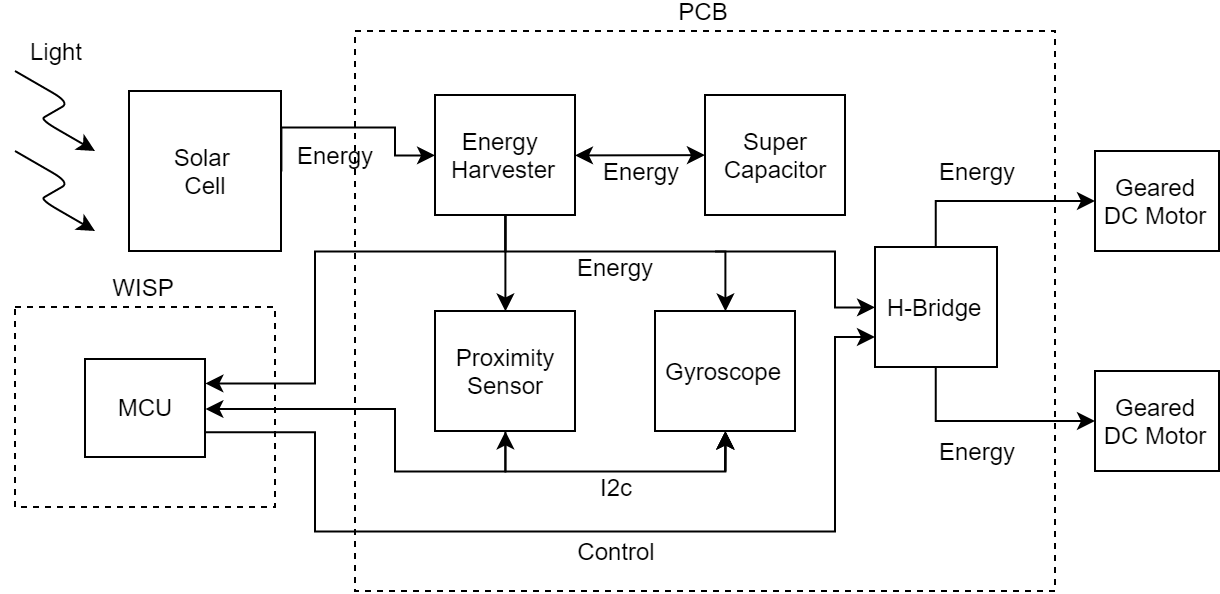
\includegraphics[width=0.9\textwidth]{pics/schematic_robot_v2.png}
	\end{figure}
\end{frame}

\begin{frame}{Robot implementation}
	\begin{figure}
		\centering
		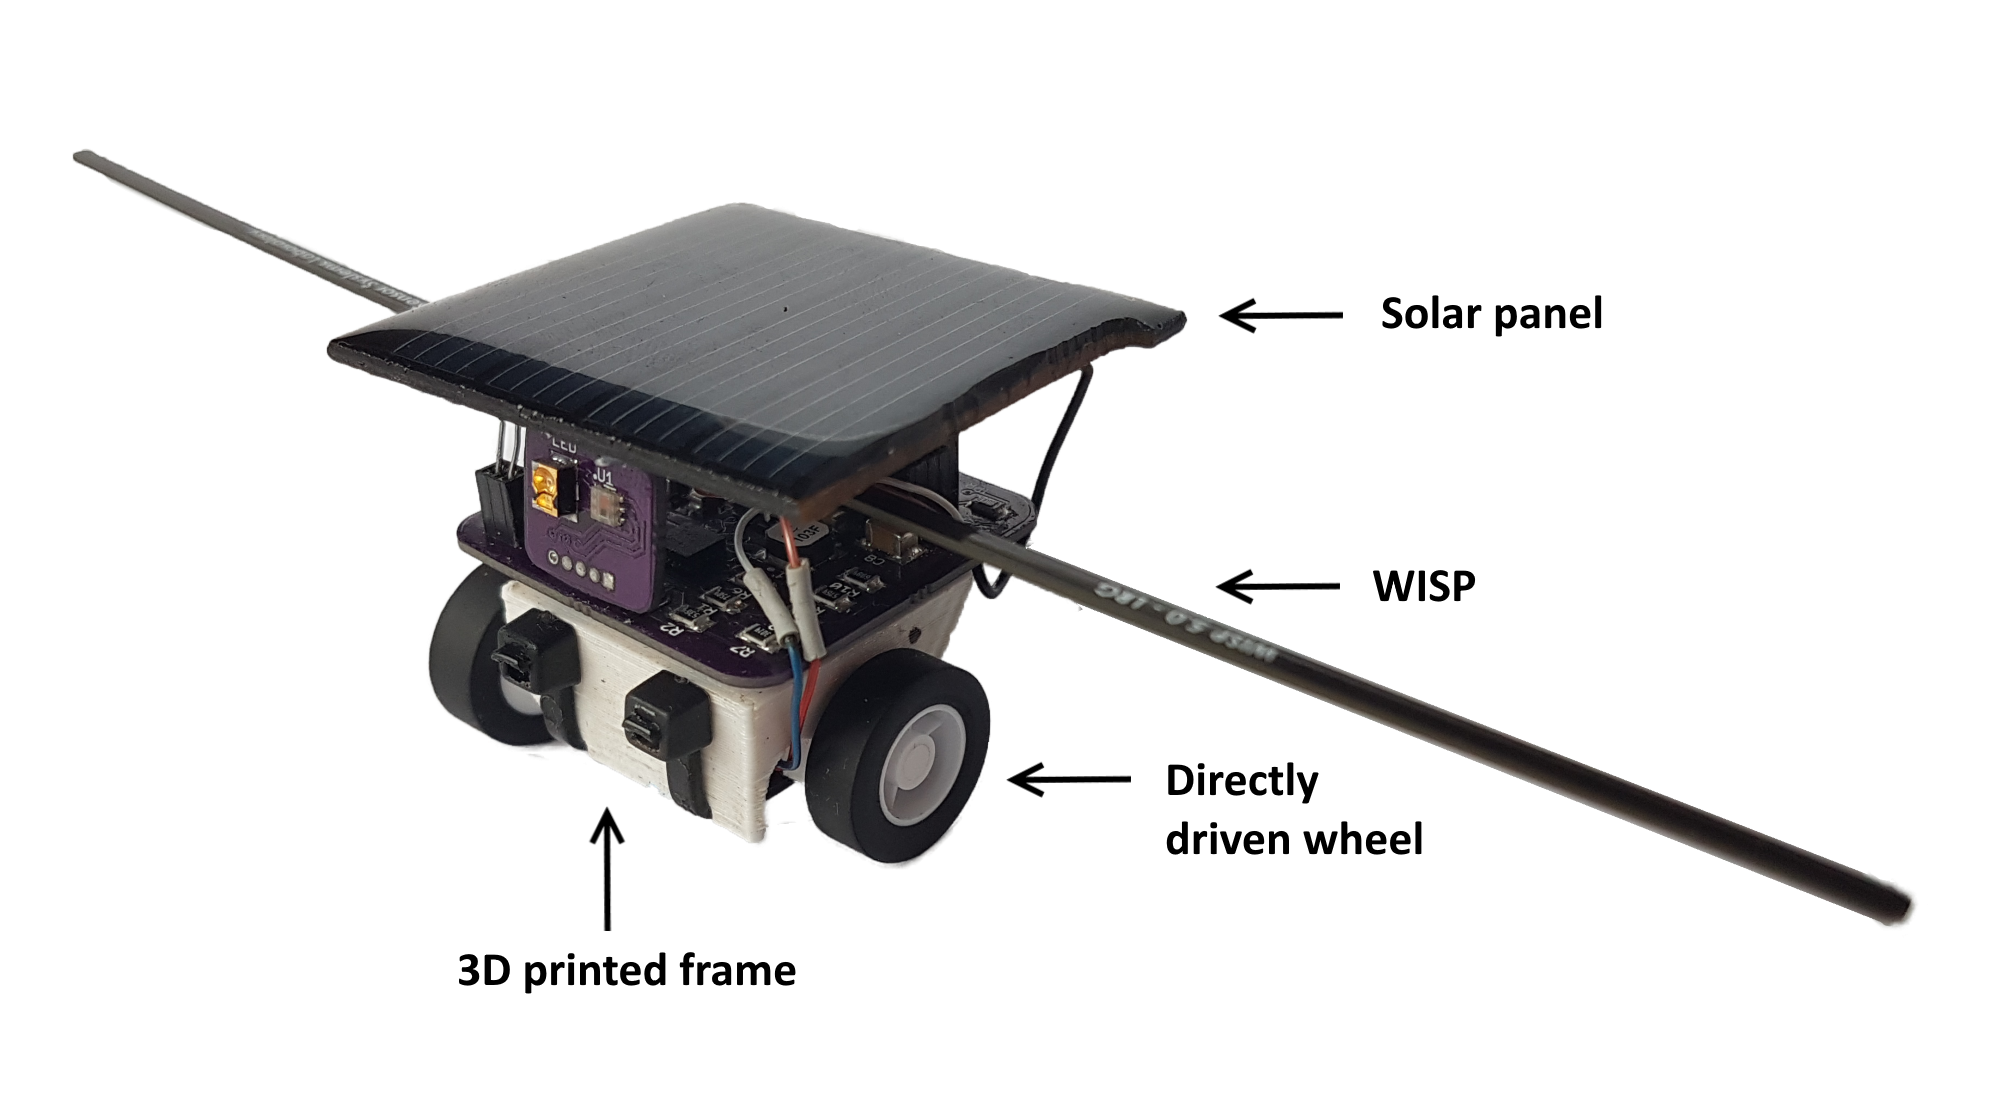
\includegraphics[width=0.9\textwidth]{pics/tp_robot2.png}
	\end{figure}
\end{frame}

\begin{frame}{Controlled movements}
	\begin{minipage}{0.45\textwidth}
		Straight and curved movements\\
		
		Yaw-rate from gyroscope \\
		
		PID controller \\
		
		Movement target \\
	\end{minipage}
	\pause
	\begin{minipage}{0.54\textwidth}\raggedleft
		\begin{figure}
			\centering
			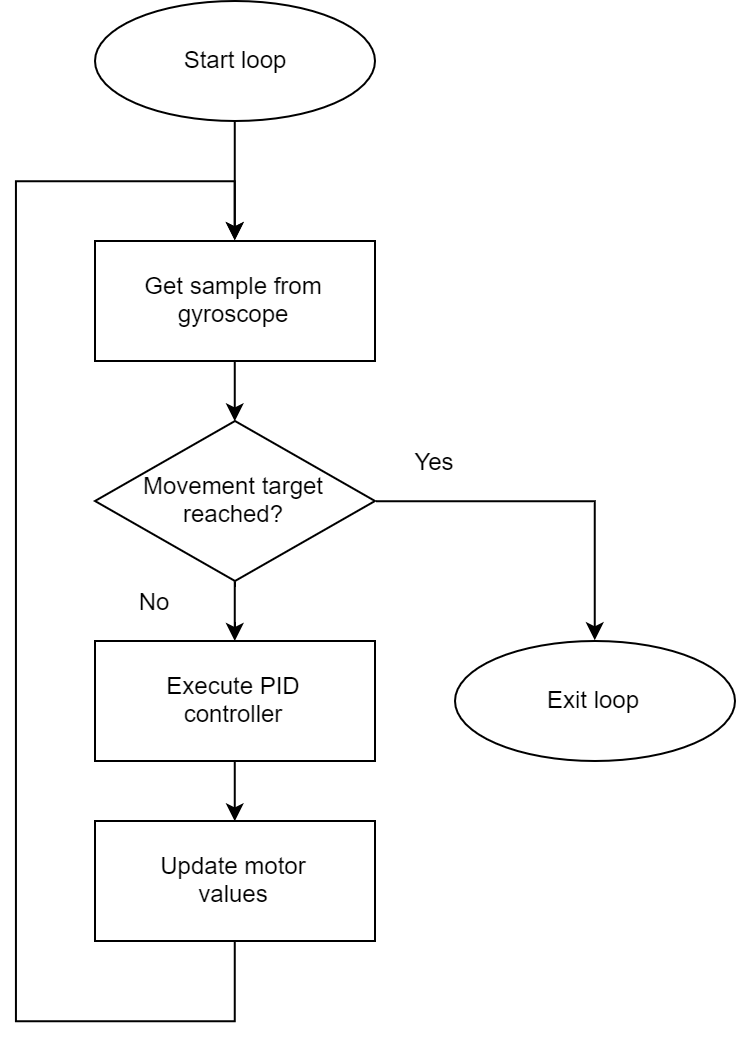
\includegraphics[width=0.8\textwidth]{pics/Flowchart_code.png}
		\end{figure}
	\end{minipage}
\end{frame}

\begin{frame}{Tuning PID controller}
	\begin{figure}
		Ziegler-Nichols Closed-Loop Tuning Method
		\begin{center}
		\begin{subfigure}[b]{0.49\textwidth}
			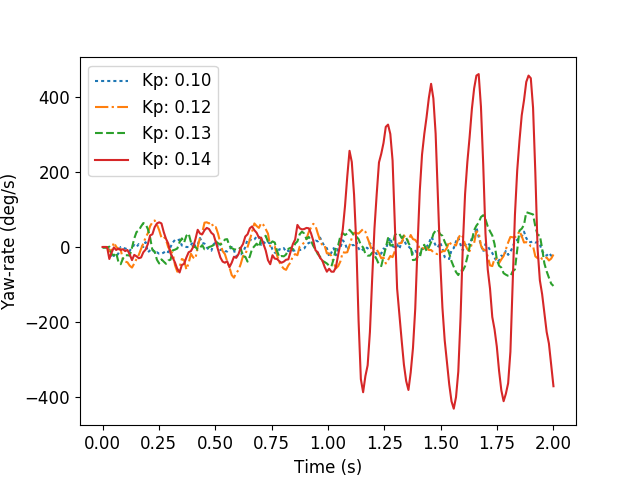
\includegraphics[width=\textwidth]{pics/straight_ku.png}
			\caption*{Determining the ultimate gain}
		\end{subfigure}
		\begin{subfigure}[b]{0.49\textwidth}
			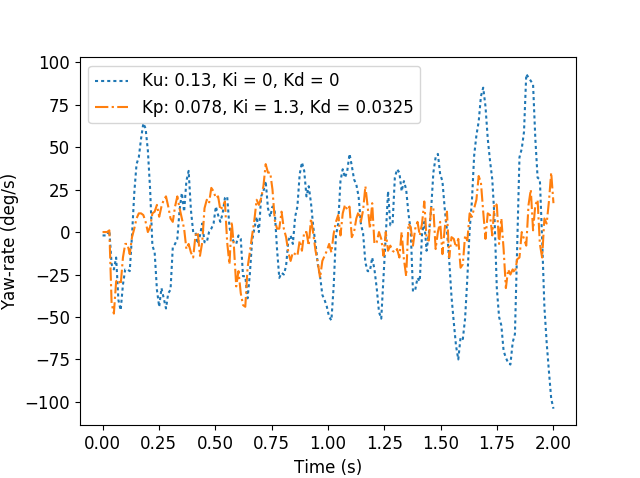
\includegraphics[width=\textwidth]{pics/straight_ku_with_tu.png}
			\caption*{Result of applying the gains}
		\end{subfigure}
		\end{center}
	\end{figure}
\end{frame}


\begin{frame}{Evaluation}
	\vspace{1em}
	\begin{figure}
		\centering
		\begin{subfigure}[b]{0.45\textwidth}
			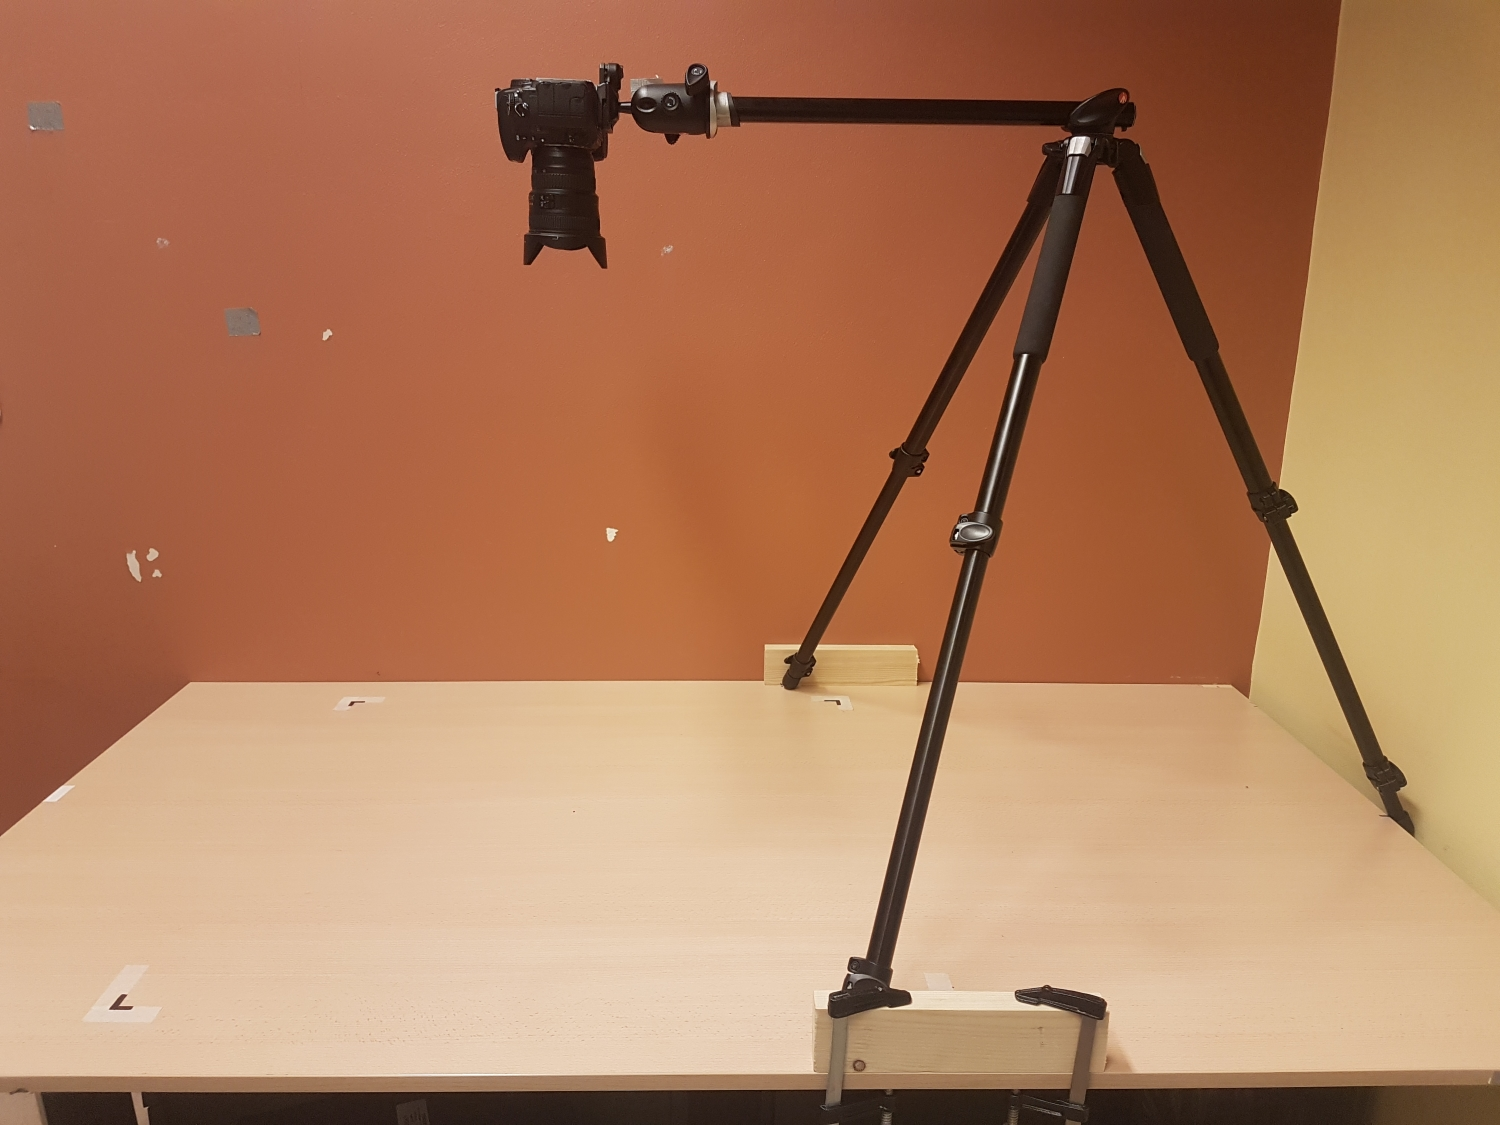
\includegraphics[width=\textwidth]{pics/movement_setup.jpg}
			\caption*{Camera setup}
		\end{subfigure}
		\quad
		\begin{subfigure}[b]{0.45\textwidth}
			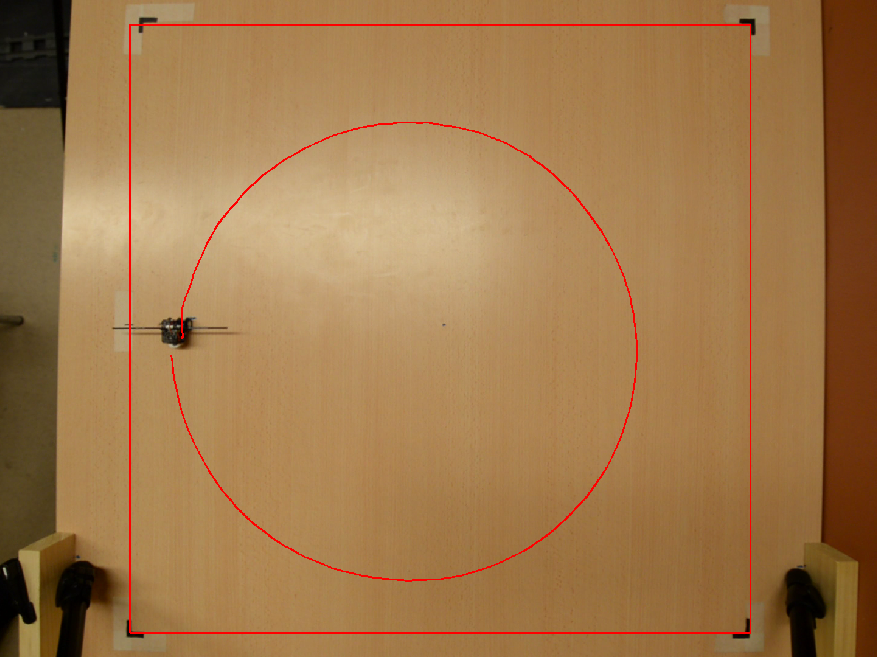
\includegraphics[width=\textwidth]{pics/movement_example.png}
			\caption*{Tracking with OpenCV}
		\end{subfigure}
	\end{figure}
\end{frame}

\begin{frame}{Minimum on time}
	\begin{figure}
		\centering
		\begin{subfigure}[b]{0.28\textwidth}
			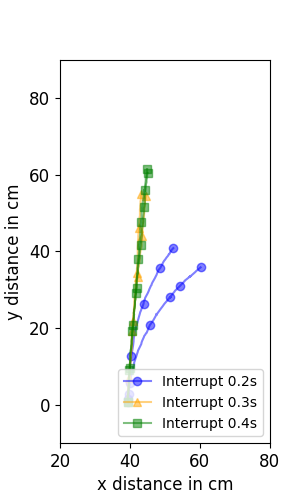
\includegraphics[width=\textwidth]{pics/figure_40.png}
			\caption*{Duty cycle 40\%}
		\end{subfigure}
		\hspace{2em}
		\begin{subfigure}[b]{0.28\textwidth}
			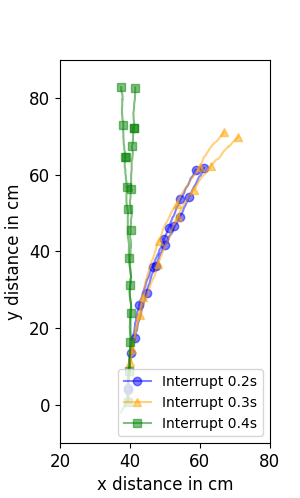
\includegraphics[width=\textwidth]{pics/figure_90.png}
			\caption*{Duty cycle 90\%}
		\end{subfigure}
	\end{figure}
	\pause
	\textbf{Conclusion:} Minimum on time $\geq$ 0.3\,s
\end{frame}

\begin{frame}{Straight movements}
	\begin{figure}
		\centering
		\begin{subfigure}[b]{0.28\textwidth}
			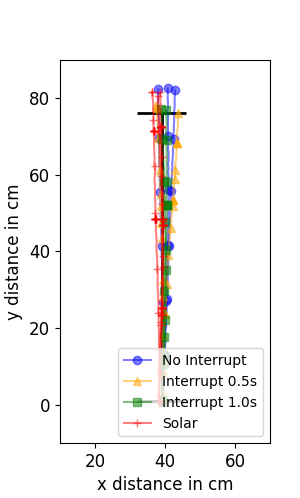
\includegraphics[width=\textwidth]{pics/straight_40.png}
			\caption*{Duty cycle 40\%}
		\end{subfigure}
		\hspace{2em}
		\begin{subfigure}[b]{0.28\textwidth}
			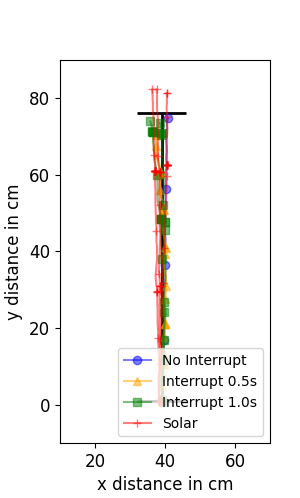
\includegraphics[width=\textwidth]{pics/straight_90.png}
			\caption*{Duty cycle 90\%}
		\end{subfigure}
	\end{figure}
	\pause
	\textbf{Conclusion:} Interrupts increase horizontal deviation
\end{frame}

\begin{frame}{Circular movements}
	\begin{figure}[h!]
		\centering
		\begin{subfigure}[b]{0.49\textwidth}
			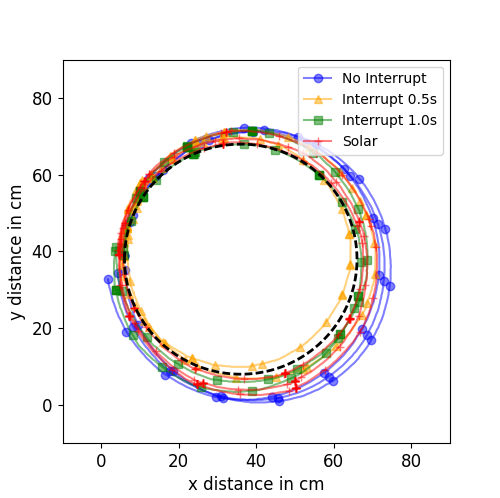
\includegraphics[width=\textwidth]{pics/circle_40.png}
			\caption*{Duty cycle 40\%}
		\end{subfigure}
		\begin{subfigure}[b]{0.49\textwidth}
			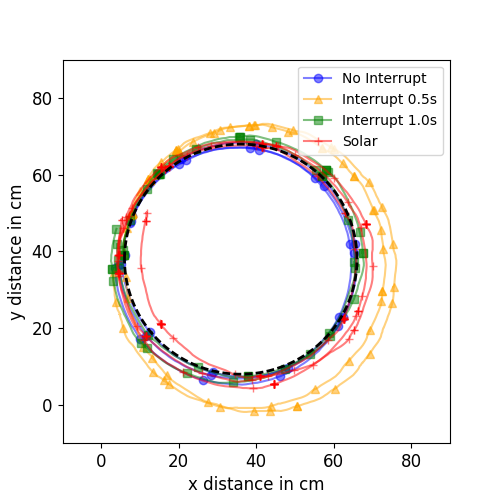
\includegraphics[width=\textwidth]{pics/circle_90.png}
			\caption*{Duty cycle 90\%}
		\end{subfigure}
	\end{figure}
	\pause
	\textbf{Conclusion:} Higher duty cycle equals less deviation from circular path
\end{frame}

\begin{frame}{Solar powered demo}
	\begin{figure}
		\centering
		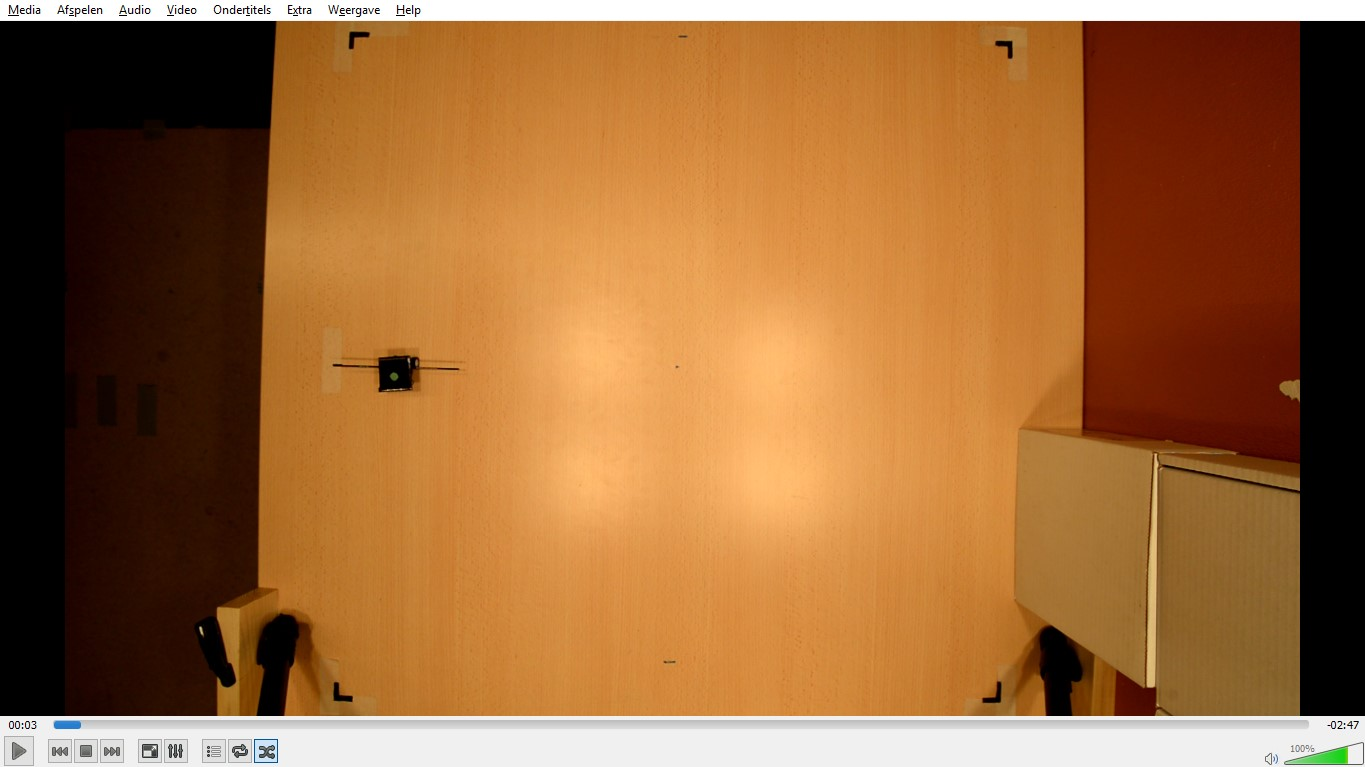
\includegraphics[width=\textwidth]{pics/video.jpg}
	\end{figure}
\end{frame}

\begin{frame}{Conclusion}
	16\% power duty cycle \\
	\vspace{1em}
	Minimum on time of 0.3\,s \\
	\vspace{1em}
	Transiently-powered vs battery-powered robot \\
	\vspace{1em}
\end{frame}

\begin{frame}{Future Work}

	Speed feedback \\
	\vspace{1em}
	Communication \\
	\vspace{1em}
	Transiently-powered swarm \\
	\vspace{1em}
	Size reduction \\
	\vspace{1em}
	Sensing capabilities \\
	
\end{frame}

\end{document}
